\chapter{Prebalené APK súbory}
\label{Repackaged}
Pojem prebalený súbor označuje APK balíčky, ktoré boli modifikované, no navonok sa prezentujú ako originálne neupravené aplikácie. Častým prípadom je, že takéto aplikácie pochádzajú z~oficiálneho zdroja Android aplikácií -- \zv{Google Play Strore}, sú upravené a následne redistribuované pomocou neoficiálnych zdrojov. Takéto aplikácie si spravidla ponechávajú dizajn a funkcionalitu originálnych aplikácií, ku ktorým však môžu pridávať nové neželané funkcie alebo modifikácie. Hlavnou motiváciou pri modifikovaní aplikácií je šírenie škodlivého softvéru – malvéru. Pozmenená aplikácia môže napríklad získať prístup k~citlivým informáciám uložených v~Android zariadení alebo monitorovať správanie užívateľa. Modifikovaná aplikácia môže obsahovať nové reklamy. Prebalovanie APK súborov má negatívny vplyv na vývojárov originálnej aplikácie. V~prípade možnosti nákupu priamo z~aplikácie\footnote{angl. in-app purchase}, môžu byť výnosy presmerované z~účtov originálnych vývojárov na účet ľudí, ktorí aplikáciu modifikovali. Ovplyvnené sú aj obchody na ktorých sa nachádzajú prebalené aplikácie, keďže používatelia uprednostnia kvalitnejšie zdroje. V~súčasnosti žiadny z~obchodov s~aplikáciami vrátane oficiálneho \zv{Google Play} nepoužíva efektívnu detekciu prebalených aplikácií~\cite{Zhauniarovich2014}. 

\section{Modifikácia APK súborov}
Modifikácia APK súborov nie je náročná. Aplikácia môže byť jednoducho rozbalená a zdrojové súbory, ako napríklad obrázky môžu byť upravené alebo nahradené inými. Štrukturovaný proces tvorby APK balíčkov~\cite{buildingAndRunning} umožňuje jednoduchú dekompiláciu. 

V~prípade modifikácie zdrojového kódu je možné použiť existujúce nástroje reverzného inžinierstva, napríklad \zv{dex2Jar} alebo \zv{ApkTool}, ktoré sú bližšie popísané v~kapitole \ref{nastroje_revezneho_inzinierstva}. 

Modifikácia súboru \zv{AndroidManifest.xml} je takisto možná. Pomocou existujúcich nástrojov je možné  previesť ho do čitateľného XML súboru, ktorý je možné editovať a následne previesť späť do binárneho XML formátu. Túto funkcionalitu poskytuje okrem iných utilít aj \zv{ApkTool}.

Android obsahuje ochranu pred narušením integrity APK balíčka, ktorá je zabezpečená pomocou súborov v~priečinku \zv{META-INF} v~koreňovej zložke APK súboru (viď \ref{META-INF}). V~prípade detekcie narušenia integrity, Android zakáže inštaláciu aplikácie. Po každej zmene súborov v~APK balíčku je nutné podpísať ho. Aplikácie sú zvyčajne podpísané certifikátom, ktorý je podpísaný identitou ktorú identifikuje\footnote{angl. self-signed certificate}. Vďaka tomu je možné po modifikácii APK balíček podpísať a zabezpečiť tak jeho fungovanie.

\section{Známe metódy detekcie prebalených APK súborov}
Jednoduchá modifikácia inštalačných balíčkov predstavuje problém pre celkový ekosystém aplikácií pre Android. Riešenie problému pozmeňovania a redistribúcie APK súborov je v~súčasnosti dôležitou témou. Bolo navrhnutých viacero spôsobov detekcie prebalených aplikácií. 

\subsection{Detekcia pomocou analýzy výkonných častí aplikácie}
Väčšina navrhnutých spôsobov detekcie modifikovaných APK balíčkov využíva metódy analyzujúce vlastnosti vyplývajúce z~vykonávaného zdrojového kódu aplikácie, spolu so súborom \zv{AndroidManifest.xml}. Úprava zdrojového kódu je nevyhnutná v~prípade editácie za účelom pridania novej neželanej funkcionality, pridania nových knižníc s~reklamou alebo editácie pôvodnej reklamy použitej v~aplikácii. Originálny zdrojový kód v~jazyku Java však nie je možné zo súboru \zv{classes.dex} extrahovať. Využíva sa zdrojový kód aplikácie vo formáte smali, ktorý je možné získať pomocou nástrojov reverzného inžinierstva (viď \ref{nastroje_revezneho_inzinierstva}). Motiváciou pre editáciu metasúboru \zv{AndroidManifest.xml} je možnosť pridávať aplikáciám prístupové povolenia (viď \ref{el_uses-permission}).
Riešenia sú založené na použití statickej analýzy kódu, dynamickej analýzy alebo na detekcii známych vzoriek škodlivého kódu\footnote{angl. signature based}~\cite{Huang2013,Chen2015,Milanova2005,Levchenko2011,Hanna2013,Zhou2012,Potharaju2012}.
	
\subsection{Detekcia pomocou podobnosti súborov}
Prebalené APK súbory je možné úspešne detekovať prostredníctvom zhody súborov obsiahnutých v~APK balíčkoch. Tento prístup využíva skutočnosť, že aplikácia nie je definovaná iba svojim zdrojovým kódom a funkcionalitou, ale je tvorená aj ďalšími dôležitými prvkami ako používateľské prostredie alebo multimediálny obsah. APK balíčky obsahujú množstvo doplnkových zdrojových súborov.  Základom tohto prístupu je pozorovanie, že modifikované aplikácie zachovávajú užívateľské rozhranie, dizajn, ikony, obrázky alebo zvuky pôvodných aplikácií. Práve tieto prvky výrazne odlišujú aplikácie, identifikujú ich pre užívateľov a majú výrazný dopad na užívateľský dojem. Preto je veľká časť súborov z~neupravených APK balíčkov obsiahnutá aj v~modifikovaných balíčkoch. Originálna aplikácia Opera Mini a verzia tejto aplikácie obsahujúca malvér, sa zhodujú v~230 z~234 súborov nachádzajúcich sa v~príslušných APK balíčkoch~\cite{Zhauniarovich2014}. Riešenie prezentované v~práci \zv{FSquaDRA}~\cite{Zhauniarovich2014} porovnáva všetky súbory medzi dvoma APK balíčkami.  Porovnávanie jednotlivých súborov na binárnej úrovni by bolo výpočtovo náročné. Preto sa na porovnanie využívajú SHA1 hashe súborov, ktoré sa nachádzajú v~súbore \zv{MANIFEST.MF} (viď \ref{MANIFEST.MF}). Podobnosť aplikácií je určená na základe \zv{Jaccard indexu}. V~práci sa rozlišujú dva typy podobných APK súborov. Aplikácie sú považované za plagiátorsky prebalené aplikácie, keď obsahujú mnoho rovnakých súborov, ale sú podpísané rôznymi certifikátmi. V~prípade veľkej zhody súborov a  identických certifikátov, sú aplikácie považované za rôzne verzie jednej aplikácie a nie sú označené ako nebezpečné. Tento spôsob porovnávania neumožňuje určiť, ktorá z~aplikácií je originálna a ktorá je pozmenená. Umožňuje však rýchlu a efektívnu detekciu modifikovaných APK súborov~\cite{Zhauniarovich2014}. 

\section{Navrhnutá metóda detekcie prebalených APK súborov}
Spôsob detekcie pozmenených APK súborov prezentovaný v~rámci tejto práce vychádza zo základov metódy prezentovanej v~článku \zv{FSquaDRA: Fast Detection of Repackaged Applications}~\cite{Zhauniarovich2014}. Prístup je založený na podobnosti súborov. Celková podobnosť aplikácií je určená na základe počtu zhodných súborov prítomných v~oboch APK balíčkoch. Účelom našej implementácie nie je simulovať detekciu prebalených inštalačných súborov pomocou metódy \zv{FSquaDRA}. Cieľom je implementovať program, ktorý na detekciu modifikovaných APK balíčkov používa podobnosť obsahu balíčkov kombinovanú s~metadátami a informáciami o~daných APK súboroch. Metadáta sú využívané na zefektívnenie výpočtu, ktoré je dosiahnuté neporovnávaním súborov medzi dvojicami zjavne odlišných aplikácií. Informácie získané porovnávaním a analýzou dvoch podobných aplikácií sú užívateľovi prezentované ako výstup porovnania. V~prípade podobnosti aplikácií je výstupom porovnania zoznam odlišností, a typ podobnosti dvoch aplikácií. Typ podobnosti je určený na základe zhody certifikátov a zhody verzií aplikácií. 
\begin{figure}[htb]
  \begin{center}
    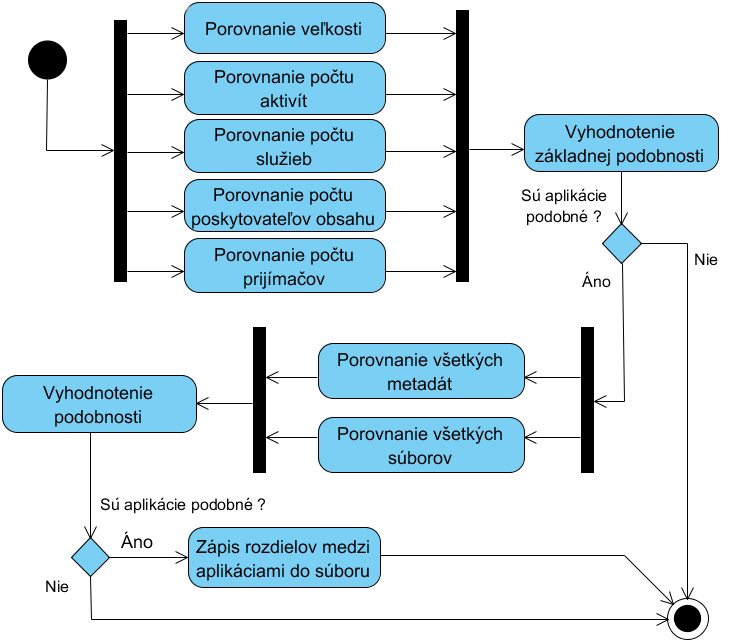
\includegraphics[height=10cm]{images/diagram.jpg}
  \end{center}
  \caption{Postup párového porovnávania APK súborov}
  \label{fig:compareFlow}
\end{figure}
\subsection{Implementácia}

Funkcionalita porovnávania a detekcie modifikovaných APK balíčkov je implementovaná v~programe \zv{ApkAnalyzer}. Používateľ môže aplikáciu spúšťať a zadávať jej parametre pomocou príkazového riadku. Funkcionalita porovnávania APK súborov sa spúšťa pomocou parametra \zv{–compare}. Vstup pre porovnávanie APK súborov nie sú samotné APK balíčky, ale JSON súbory, ktoré sú vytvorené aplikáciou \zv{ApkAnalyzer} počas analýzy APK balíčkov a obsahujú metadata o~aplikáciách (viď kapitola \ref{analyza}). Samotné porovnávanie prebieha párovo, každá aplikácia je porovnávaná so všetkými ostatnými. Proces porovnávania je paralelizovaný a každé dostupné procesorové jadro porovnáva inú dvojicu aplikácií. 

Porovnávanie a vyhodnocovanie podobnosti je rozdelené do viacerých etáp. Najskôr sa porovnávajú základné informácie o~APK súboroch a príslušných aplikáciách. Toto porovnanie využíva základné metadáta o~aplikáciách a zahŕňa veľkosť APK súboru, počet komponent z~ktorých sa aplikácia skladá (aktivity, služby, poskytovatelia obsahu, prijímače), počet rôznych obrázkových súborov a počet súborov definujúcich vzhľad obrazoviek.

Všetky tieto hodnoty sú číselné. Je nutné aby implementácia ich porovnávania bola funkčná nezávisle na veľkosti týchto číselných hodnôt. Taktiež je nutné zabezpečiť komutatívnosť, ktorá zaručí, že nezáleží na poradí porovnávania aplikácií a teda pre funkciu porovnávania $func$ platí \[func(A,B) = func(B,A)\] Získané hodnoty sú porovnávané s~minimálnymi hodnotami potrebnými na to, aby boli aplikácie považované za podobné. Tieto hodnoty je možné meniť editáciou súboru \zv{similarity.properties} v~koreňovej zložke projektu \zv{ApkAnalyzer}.

V~prípade detekcie základnej podobnosti sa porovnajú všetky súbory v~APK balíčkoch. Podobne ako v~aplikácií vyvinutej v~rámci projektu \zv{FSquaDRA}, na porovnanie sú využité SHA1 hashe súborov uložené v~\zv{MANIFEST.MF}. Separátne sú porovnávané súbory \zv{classes.dex}, \zv{resources.arsc}. Ostatné súbory sú porovnávané v~rámci kategórií: obrázkové súbory, súbory definujúce vzhľad obrazoviek a všetky ostatné súbory. Z dôvodu jednoduchšej práce s výstupom porovnania je spočítaný aj agregovaný rozdiel všetkých súborov v~APK balíčku. 

Zhoda súborov medzi dvomi APK balíčkami je určená pomocou Jaccardovho koeficientu podobnosti~\cite{Phillips2013}. Nech $A$ sú súbory v~danej kategórií v~jednom APK balíčku, $B$ sú súbory v~danej kategórií v~druhom porovnávanom APK balíčku. \[Jaccard Index(A,B) = \frac{|A~\cap B|}{ |A~\cup B|}\] Aplikácie sú považované za podobné v~prípade, že hodnota koeficientu podobnosti pre každú z~kategórií súborov v APK balíčku prekračuje minimálnu hodnotu definovanú v~súbore \zv{similarity.properties}. Určenie podobnosti v~tejto fáze prebieha len na základe rovnakých súborov. Okrem súborov sa porovnajú aj všetky hodnoty metadát získaných analýzou APK súboru. Tieto hodnoty sú použité ako informácie v detailnom výstupe porovnania.

\paragraph{Typ podobnosti}\mbox{}\\
Zhoda certifikátov a zhoda verzií aplikácií je vypočítaná za účelom určenia typu podobnosti daných aplikácií. Pri zhode verzií a certifikátov rozlišuje tri hodnoty – rovnaké, rozdielne alebo neurčené. Hodnota neurčené je použitá v~prípade, že sa dáta nepodarilo získať. Zhoda certifikátov sa určuje na základe hashu certifikátu. Tento údaj je v~kontexte detekcie modifikovaných APK súborov veľmi dôležitý. V~prípade zhody certifikátov je zaručené, že APK súbory pochádzajú od rovnakého vydavateľa. Pokiaľ sú certifikáty rozdielne, pôvodca súborov je s~najväčšou pravdepodobnosťou rozdielny. Zhoda verzií aplikácií je využitá na detekciu rovnakých aplikácií v~rozdielnych verziách.
Kombinácia týchto hodnôt určuje 9 kategórií podobnosti APK súborov. Každá z~týchto kategórií napovedá a vzájomnom vzťahu danej dvojice Android aplikácií. Najväčšia pravdepodobnosť, že aplikácia je prebalená, je v~prípade rovnakých verzií a zároveň rozdielnych certifikátov. 

\paragraph{Výstup porovnania}\mbox{}\\
V~prípade, že porovnávaná dvojica APK súborov je vyhodnotená ako podobná, \zv{ApkAnalyzer} vytvorí výstupný súbor vo formáte JSON obsahujúci rozdiely medzi danými aplikáciami. Tento súbor obsahuje rozdiely určené na základe metadát a porovnania aplikácií. Slúži ako jednoduchá obdoba linuxového príkazu \zv{diff} implementovaná nad APK súbormi. Obsahuje informácie o~modifikovaných parametroch a komponentoch aplikácií a taktiež zoznam upravených, nových alebo odstránených súborov. Zjednodušený príklad vzorového výstupného súboru obsahuje ukážka 7.1.
\begin{lstlisting} [language=json, caption= {Zjednodušená ukážka výstupu párového porovnanie APK súborov} \label{json:compare}]
{
  "nameA": "SoundHound  v6.7.5 apakrchive.com.apk",
  "nameB": "SoundHound 8 v6.3.3.apk",
  "hashCompareResult": {
    ...
    "modifiedDrawableFiles": [
      "res/drawable-nodpi-v4/ic_action_help.xml",
      ...
    ],
    "additionalDrawableFilesA": [
      "res/drawable-hdpi-v4/com_facebook_button_like_icon_selected.png",
      ...
    ],
    "additionalDrawableFilesB": [
      "res/drawable-hdpi-v4/ic_timestamp_clock_10dp.png",
      ...
    ],
    ...
  },
  "metadataCompareResult": {
    "fileSizeDifference": {
      "count": -2899397,
      "percentage": 16.98035514829626890787039883434772491455078125
    },
    "packageName": {
      "isSame": true
    },
    "versionCode": {
      "isSame": false,
      "difference": {
        "valueA": "10675",
        "valueB": "10633"
      }
    },
    "additionalActivitiesInA": [
      "com.soundhound.android.appcommon.activity.SplashScreenActivity",
      ...
    ],
    ...
  }
}
\end{lstlisting}

\subsection{Výsledky}
Vyhľadávanie možných prebalených APK súborov pomocou navrhnutej metódy určilo v~našej databáze viacero podozrivých aplikácií. Porovnávanie všetkých aplikácií v~našej databáze znamenalo viac ako dva milióny vykonaných párových porovnaní. Celkový čas potrebný na výpočet dosiahol približne 40 hodín. Porovnanie bolo vykonané na výkonnom ale bežnom komoditnom harvéri\footnote{Procesor Intel Core i7-4900MQ @ 2.80GHz , 16GB RAM, SSD disk}. V~čase potrebnom na porovnanie nie je započítaný čas na analýzu APK súborov a vytvorenie JSON súborov obsahujúcich metadáta. Vzhľadom na objem zbieraných dát a dekompiláciu APK balíčku pomocou nástroja \zv{ApkTool} počas analýzy (viď kapitola \ref{analyza}), je celkový čas potrebný na určenie prebalených súborov vyšší ako v~prípade metódy \zv{FSquaDRA}, avšak výstup nášho porovnania obsahuje informácie o~rozdieloch medzi jednotlivými APK súbormi. Dvojica APK súborov je považovaná za nadmieru podobnú v~prípade splnenia konfigurovateľných ktirétií podobnosti. Tie boli počas porovnávania nastavené na minimálnu zhodu 50\,\%, respektíve hodnotu \zv{Jaccard indexu} 0,5. Veľké množstvo aplikácií bolo vyhodnotených ako podobné, lebo sa jednalo o~rovnaké aplikácie v~rozdielnych verziách. Takéto aplikácie je možné vyfiltrovať s~využitím kategórie podobnosti, ktorá je každej porovnávanej dvojici priradená. \zv{ApkAnalyzer} automaticky rozdelí výstupné súbory do podpriečinkov podľa typu podobnosti APK súborov. Bolo identifikovaných 161 dvojíc aplikácií, ktoré splňovali kritériá zhody, boli v~rovnakej verzii, ale boli podpísané rôznymi certifikátmi.